\documentclass{article}
\usepackage{enumerate}
\usepackage{amsmath}
\usepackage{amssymb}
\usepackage{graphicx}
\usepackage{subfigure}
\usepackage{geometry}
\usepackage{caption}
\usepackage{stmaryrd}
\geometry{left=3.0cm,right=3.0cm,top=3.0cm,bottom=4.0cm}
\renewcommand{\thesection}{Problem \arabic{section}.}
\title{VP260 PROBLEM SET 11}
\author{Liu Yihao 515370910207}
\date{}
\begin{document}
\maketitle

\section{}
\begin{enumerate}[(a)]
\item
$$U=\bar{E}d=\bar{I}R=I\frac{\rho d}{\pi a^2}\hat{n_I}$$
$$\bar{E}=\frac{\rho I}{\pi a^2}\hat{n_I}$$
$$\bar{B}=\frac{\mu_0I}{2\pi a}\hat{n_\theta}$$
\item
$$S=\frac{1}{\mu_0}(\bar{E}\times\bar{B})=-\frac{\rho I^2}{2\pi^2a^3}\hat{n_r}$$
\item
$$\frac{dE}{dt}=-S\cdot 2\pi al=\frac{\rho lI^2}{\pi a^2}$$
\item
$$\frac{dQ}{dt}=P=I^2R=I^2\frac{\rho l}{\pi a^2}=\frac{\rho lI^2}{\pi a^2}$$
So they are the same, because energy in the conductor is transformed into heat so that it should obtain energy from outside in preserve the constant current $I$.
\end{enumerate}

\section{}
Suppose the incident angle of ray $A$ is $\theta$, then the reflection angle of $A$ is $\theta$ and the refraction angle of $A$ is $\dfrac{n_1}{n_2}\theta$. The reflection angle of the refraction ray is also $\dfrac{n_1}{n_2}\theta$. When the refraction ray refracts again, the refraction angle is $\dfrac{n_2}{n_1}\dfrac{n_1}{n_2}\theta=\theta$, which is same as the reflection angle of $A$, so they are parallel to each other.

\section{}
Suppose the initial direction is $x\hat{n_x}+y\hat{n_y}+z\hat{n_z}$.\\
If it reflects on the xy-plane, the direction of z-axis will become opposite.\\
If it reflects on the xz-plane, the direction of y-axis will become opposite.\\
If it reflects on the yz-plane, the direction of x-axis will become opposite.\\
So when the ray reflects on all of the three planes, the final direction is $-x\hat{n_x}-y\hat{n_y}-z\hat{n_z}$, which is opposite to the initial direction.

\section{}
\begin{enumerate}[(a)]
\item
We can't directly rotate $90^\circ$ since $I_0\cos^290^\circ=0$, so at least two sheets are required.
\item
$$I_0\prod_{i=1}^n\cos^2\theta_i\geqslant0.6I_0$$
$$\prod_{i=1}^n\cos\theta_i\geqslant\sqrt{0.6}$$
According to fundamental inequality,
$$\prod_{i=1}^n\cos\theta_i\leqslant\frac{1}{n}\left(\sum_{i=1}^n\cos\theta_i\right)^n$$
if and only if $\theta_1=\theta_2=\cdots=\theta_n$, it gets the maximum.\\
And we know $\sum_{i=1}^n\theta_i=90^\circ$, so $\theta_i=\frac{90}{n}^\circ$
$$\cos^n\frac{90}{n}^\circ\geqslant\sqrt{0.6}$$
$$n\geqslant5$$
so at least five sheets are required.

\end{enumerate}

\section{}
If $|PS_2|-|PS_1|=m\lambda,m\in Z\backslash\lbrace0\rbrace$, it is hyperbola.\\
If $|PS_2|-|PS_1|=\frac{2m+1}{2}\lambda,m\in Z\backslash\lbrace0\rbrace$, it is hyperbola.\\

\section{}
\begin{enumerate}[(a)]
\item
$$E_1=E\cos(kr-\omega t)$$
$$E_2=2E\cos(kr-\omega t+\varphi)$$
\begin{align*}
E_1+E_2&=E\cos(kr-\omega t)(2\cos\varphi+1)-2E\sin(kr-\omega t)\sin\varphi\\
&=E\sqrt{(2\cos\varphi+1)^2+(2\sin\varphi)^2}\sin\left(-\arctan\frac{2\cos\varphi+1}{2\sin\varphi}\right)\\
&=E\sqrt{5+4\cos\varphi}\sin\left(-\arctan\frac{2\cos\varphi+1}{2\sin\varphi}\right)
\end{align*}
$$I=\frac{E_0^2}{2\mu_0c}=\frac{E^2}{2\mu_0c}(5+4\cos\varphi)$$
$$I_{max}=\frac{9E^2}{2\mu_0c}$$
$$I=I_{max}\left(\frac{5}{9}+\frac{4}{9}\cos\varphi\right)$$
\newpage
\item \ 
\begin{figure}[!h]
\centering
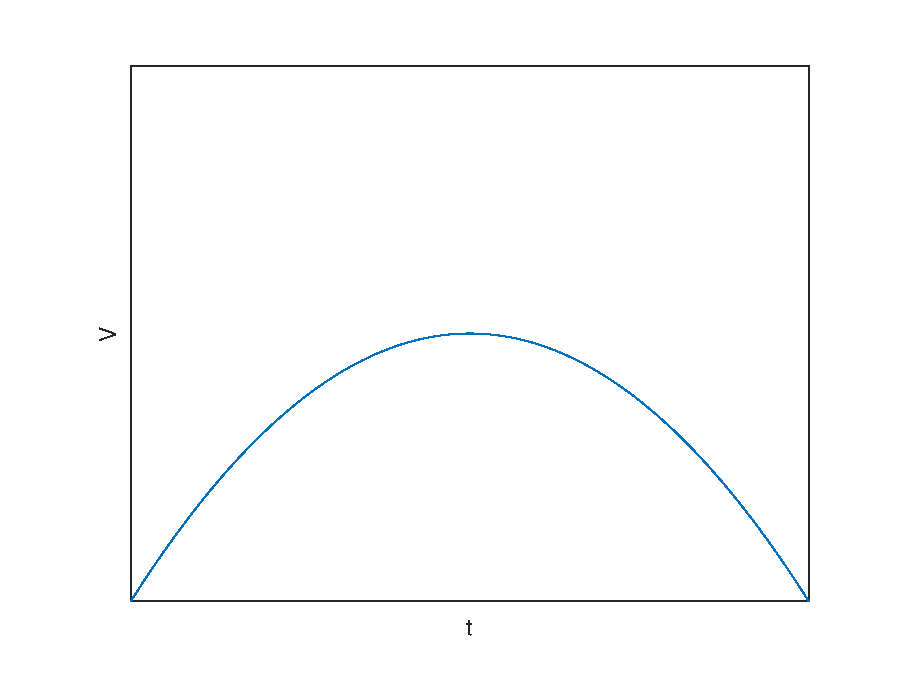
\includegraphics[scale=0.5]{1.eps}
\end{figure}
$$I_{min}=\frac{1}{9}I_max$$
$$\varphi=(2k+1)\pi,k\in Z$$
\end{enumerate}

\section{}
$$I_{max}\cos^2\frac{\pi dy}{\lambda l}=\frac{1}{2}I_{max}$$
$$\cos\frac{\pi dy}{\lambda l}=\pm\frac{\sqrt{2}}{2}$$
$$\frac{\pi dy}{\lambda l}=\frac{(2k+1)\pi}{4},k\in Z$$
$$y=\frac{(2k+1)\lambda l}{4d}$$
For every k,
$$\Delta\theta_m=\frac{\Delta y}{l}=\frac{\lambda}{2d}$$
It doesn't depend on $m$.

\section{}
$$r_2-r_1=\frac{\lambda}{2}$$
$$2nh=\frac{\lambda}{2}$$
$$h=\frac{\lambda}{4n}=109.72\,\rm nm$$

\end{document}
